% Chapter 2
\let\cleardoublepage\clearpage
 % \let\cleardoublepage\clearpage
\chapter{Literature Review} % Main chapter title

\label{Chapter2} % For referencing the chapter elsewhere, use \ref{Chapter1} 

%----------------------------------------------------------------------------------------

% Define some commands to keep the formatting separated from the content 
\newcommand{\keyword}[1]{\textbf{#1}}
\newcommand{\tabhead}[1]{\textbf{#1}}
\newcommand{\code}[1]{\texttt{#1}}
\newcommand{\file}[1]{\texttt{\bfseries#1}}
\newcommand{\option}[1]{\texttt{\itshape#1}}

\section{Overview of Credit Card Fraud Detection}

Credit card fraud represents a persistent and evolving threat in the financial ecosystem, where malicious actors seek to exploit vulnerabilities in payment systems for personal gain. This section provides an insightful overview of credit card fraud, shedding light on the tactics employed by fraudsters and the dynamic landscape of fraudulent activities.



Credit card fraud manifests in various forms, including:\medskip 
\begin{itemize}
    \item According to the Nilson Report, global card fraud losses were estimated to be around \$27.85 billion in 2018.\medskip 

    \item  The Federal Trade Commission (FTC) reported that credit card fraud represented a significant portion of identity theft cases, with around 33\% of all reported cases in 2020.\medskip 

    \item According to Visa, merchants who have completed the EMV chip upgrade saw a 76\% drop in counterfeit fraud from December 2015 to March 2018.\medskip 

    
    
    \item  The LexisNexis True Cost of Fraud Study 2019 reported that for every dollar of fraud, merchants incurred an additional \$3.13 billion in costs.\medskip

    \item  Depending on the complexity and the dataset used, have reported accuracies ranging from 85\% to 99\%.\medskip

    \item  Balancing the detection of fraudulent activity with minimizing false positives is a constant challenge. False positive rates for some models have been reported in the range of 1\% to 5\%.\medskip
\end{itemize}

\subsection{Evolution of Credit Card Fraud:}

As technology advances, so do the methods employed by fraudsters. The emergence of online transactions and digital payment methods has introduced new vectors for exploitation, necessitating innovative and adaptive fraud detection measures.\medskip

Understanding the multifaceted nature of credit card fraud is crucial for developing effective detection systems that can anticipate and thwart the ever-changing strategies of malicious actors. In the subsequent sections, we delve into the existing methods and the application of machine learning, particularly the Random Forest Classifier, to fortify credit card fraud detection mechanisms.






%----------------------------------------------------------------------------------------

\section{Existing Fraud Detection Methods}

\subsection{Random Forest}

Random forest is a type of supervised machine learning
algorithm based on ensemble learning. Ensemble learning is
a type of learning where you join different types of
algorithms or same algorithm multiple times to form a more
powerful prediction model. The random forest algorithm
combines multiple algorithm of the same type i.e. multiple
decision trees, resulting in a forest of trees, hence the name
"Random Forest". The random forest algorithm can be used
for both regression and classification tasks.\medskip

\keyword{WORKING OF RANDOM FOREST } 
\begin{itemize}
\item 1. Pick N random records from the dataset.
\item 2. Build a decision tree based on these N records.
\item 3. Choose the number of trees you want in your
algorithm and repeat steps 1 and 2.
\item 4. For classification problem, each tree in the forest
predicts the category to which the new record belongs.
Finally, the new record is assigned to the category that
wins the majority vote..\medskip
\end{itemize}
\keyword{Advantages of using Random Forest}
\begin{itemize}
\item  The random forest algorithm is not biased, since,
there are multiple trees and each tree is trained on a
subset of data. Basically, the random forest algorithm
relies on the power of "the crowd"; therefore, the
overall biasedness of the algorithm is reduced.
\item  This algorithm is very stable. Even if a new data
point is introduced in the dataset the overall algorithm
is not affected much since new data may impact one
tree, but it is very hard for it to impact all the trees.
\item  The random forest algorithm works well when you
have both categorical and numerical features.

\subsection{Logistic Regression}
Logistic regression is another powerful supervised ML algorithm used for binary classification problems (when target is categorical). The best way to think about logistic regression is that it is a linear regression but for classification problems. The primary difference between linear regression and logistic regression is that logistic regression's range is bounded between 0 and 1. In addition, as opposed to linear regression, logistic regression does not require a linear relationship between inputs and output variables.Logistic regression is based on the sigmoid function and its result is from zero to one. 
\medskip
\begin{figure}[h]
    \centering
    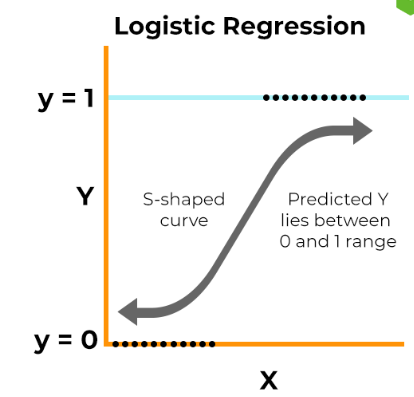
\includegraphics[width=0.5\linewidth]{image1.png}
    \caption{Logistic Regression}
    \label{fig:enter-label}
\end{figure}
\keyword{Advantages of using Logistic Regression}
\item Logistic regression provides easily interpretable results. The coefficients assigned to each feature indicate the strength and direction of their influence on the likelihood of fraud. This transparency is crucial for understanding the factors contributing to fraud.

\item It's computationally efficient, especially when compared to more complex models. This efficiency becomes important when dealing with large datasets, a common scenario in credit card transactions.

\item Credit card fraud detection is essentially a binary classification problem (fraud or not fraud). Logistic regression is specifically designed for such scenarios and is well-suited for predicting probabilities associated with two outcomes.
\item If the data can be separated by a straight line (or hyperplane in higher dimensions), logistic regression performs well. In many cases, fraud detection features may exhibit a linear relationship with the likelihood of fraud, making logistic regression a suitable choice.





\end{itemize}
